\subsection{Method and Implementation}
As described in Section \ref{lasso-back}, LASSO is a regression technique that finds weights applied to an input to produce a known output. This technique can also work on noisy outputs and thus can be applied to channel reconstruction of sparse channels. The channel is modeled in the form of:

\[ y = \Psi h + n \]

Where $y$ is the received signal, $\Psi$ is the transmitted reference signal containing the sequence of pilot symbols, $h$ is the channel vector and the main component used for channel reconstruction, and $n$ is the noise of the channel between two communicating entities \cite{Tse2004}. In the case of LASSO regression for channel sounding the transmitted and received reference signals can be converted into their angular domain representation using the Inverse Discrete Fourier Transform of the transmitted signal or by using the following transform from \cite{Tse2004}:

\[ \Psi^a = U_t \Psi \]

\[ U_t(k,l) = \dfrac{1}{\sqrt{n_t}} exp(\dfrac{-j2\pi k l}{n_t}) \] 

Where $n_t$ is the number of transmit antennas in our MIMO Uniform Linear Array (ULA) of antennas. $U_t$ is a unitary matrix that is $n_t \times n_t$, and $k$ and $l$ are the row and column indices of the square $U_t$ matrix \cite{Tse2004}. $U_t$ represents the matrix to preform the Inverse Discrete Fourier Transform on the transmitted signal $\Psi$ to yield the angular domain representation of the signal.

LASSO sends the reference signals from the MIMO BS station to the UE in evaluation to preform channel sounding. The UE will then send the compressed received reference signal back to the BS for further processing and channel estimation \cite{Liu2016}. This method is used for two main reasons. The first is to reconstruction the downlink channel between the BS and the UE, so the reference signal should be transmitted from the BS to the UE to estimate the downlink channel. Secondly, depending on the channel sounding technique used, the power and processing resources required to reconstruction the estimate of the channel vector can be expensive. This is especially impactful for wireless UE devices that run on batteries and have limited computing power or lack specific hardware to decrease the running times of the reconstruction techniques.

Using the CDL simulator described in Section \ref{sim}, the LASSO approach to channel reconstruction transmits the reference signal from a multi-antenna ULA at the simulated BS to a UE device with one antenna. The received signals are them assumed to be transmitted back to the BS for channel sounding using the LASSO technique. In reality, the received signal at the UE would be compressed and sent back to the BS for further processing and incur heavy overheads.

As mentioned in the background section, the LASSO technique needs some modifications to it's algorithm as the input to LASSO are not real values, but complex ones. Due to this fact, a different method is needed to convert the complex valued LASSO optimization problem into a real one. There were two methods explored to complete this. The first method rearranges the real and imaginary into a new real matrix which can be solved using the normal LASSO algorithm that is built into MATLAB. The second technique uses a third party LASSO solver to solve complex valued problems. The first method seemed to yield unclear results with a high degree of error, so a third party LASSO solver was the method of choice. To accomplish this goal, a complex LASSO solver was taken from the work of Mark Schmidt's PhD work \cite{Schmidt2020}. The LASSO solver combines methods of the first method, by rearranging the complex values into a mapped real matrix of values, and then uses a group solver to determine the sparse channel vector connecting the transmitted reference signal to the received signal before converting the values back to complex.

To calculate the error of the estimated channel vector a Normalized Mean Squared Error (NMSE) measurement is used and can be represented by the following equation:

\[ \mathrm{NMSE} = \dfrac{1}{M} \sum_{i=1}^{M} | y - \Psi h |^2 \]

\noindent
Where $M$ is the number of pilot symbols in the transmitted and received reference signal, $y$ is the received signal, $\Psi$ is the transmitted signal, and $h$ is the estimated channel vector. The difference between the actual and estimated received signals is taken and then the magnitude of the difference is squared and finally averaged by dividing the sum by the number of pilot symbols used. $M$ is also the length of the received signal as the UE only contains one antenna in our scenario. It is important to note that some error will always exist because the noise of the channel is not captured in the error equation. Therefore, the NMSE also captures the noise of the channel. Another technique that could be used to estimate the error of the channel vector could be to determine the exact channel vector and compare that directly to the estimated channel vector generated by the channel sounding technique in question. 

\subsection{Results}
\begin{figure}[H]
    \subfigure[]{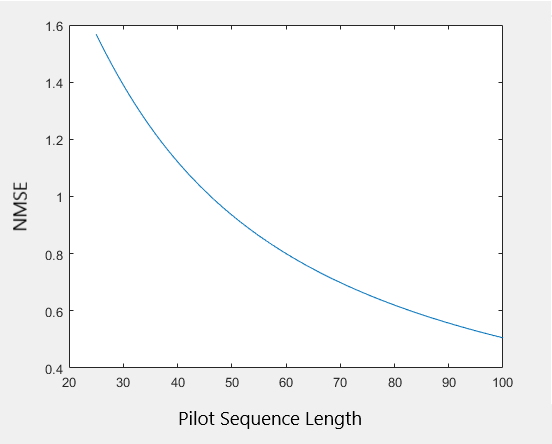
\includegraphics[width=0.45\textwidth]{MarkSchmidt-LASSO-absMSEvsPilotCount-2.PNG}}
    \subfigure[]{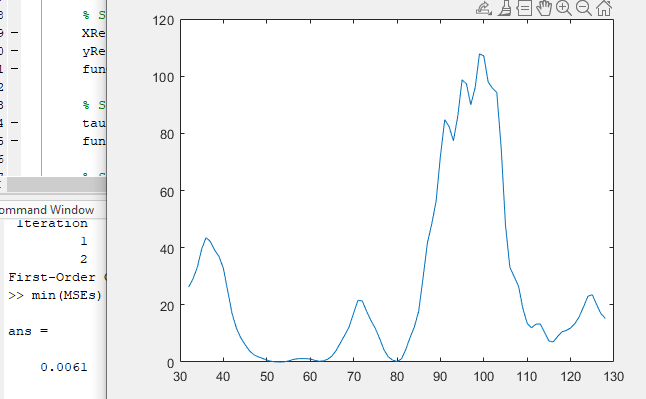
\includegraphics[width=0.45\textwidth]{MarkSchmidt-LASSO-absMSEvsAntennaCount.PNG}} 
    \caption{Results from LASSO Channel Reconstruction (a) NMSE vs. Pilot Count (b) NMSE vs. Antenna Count}
    \label{fig:lasso}
\end{figure}

Figure \ref{fig:lasso} displays the results from our MATLAB implementation of the LASSO channel estimation technique. The figures plot the NMSE versus the independent MIMO parameters, number of pilot symbols and number of antennas in a ULA. As expected, as the number of pilot symbols increases in the reference signal, the error of our estimated channel vector decreases at an exponential rate. This affirms the belief that the accuracy of the channel vector is directly proportional to the number of pilot symbols used in the reference signal sent to a UE in downlink channel reconstruction. The second image of Figure \ref{fig:lasso} shows the NMSE versus the number of antennas in a ULA. The function of number of antennas to the strength of channel estimation using the LASSO technique does not fit a common or known function. It provides an interesting insight into how the number of antennas may affect the accuracy of the LASSO technique for sparse channels. There are several peaks in the function between 30 to 50, 65 to 80, and 80 to 110 antennas. Each peak region represents ranges of antennas which produce poor channel vector estimations while using the LASSO technique. The minimum points are probably the areas of most interest as they provide insight into how many antennas are reasonable to maintain a low error of the estimated channel vector. m-MIMO systems that use LASSO channel reconstruction and have a number of antennas between 50 and 65, or 80 produce the best estimations of the channel vector. The second image used a static 50 pilot symbols to produce the following plot.

\begin{figure}[H]
\centering
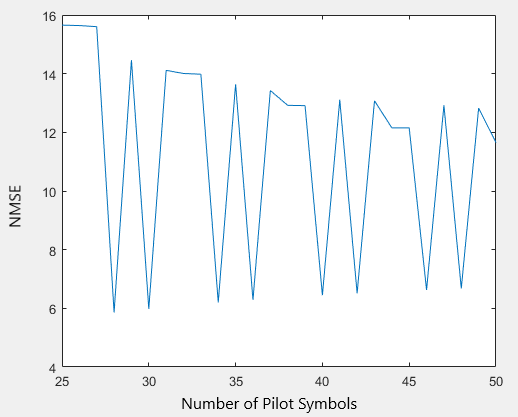
\includegraphics[width=0.5\textwidth]{figures/StackEx-LASSO-absMSEvsPilotCount.PNG}
\caption{Results from LASSO Channel Reconstruction using first method}
\label{fig:lasso-wrong}
\end{figure}

As discussed above, the first method of rearranging the complex values of the LASSO optimization problem into a real valued problem and then using MATLAB's default LASSO algorithm does not produce the expected results. Figure \ref{fig:lasso-wrong} displays the results for the NMSE versus the number of pilot symbols in the transmitted reference signals. As one can observe, the NMSE decreases irregularly as the number of pilot symbols increases. The function is quite sporadic and the does not produce results consistent with other publications \cite{Liu2016}. Therefore, this method is disregarded as it is believed something is missing or has gone wrong in the algorithm.

\subsection{Discussion}

The first method for a complex LASSO algorithm described above failed in a few different ways and can't be used as a LASSO channel sounding technique because of the large NMSE error and inconsistent results with other published works for the same technique. This leads the authors to believe that there is an implementation issue for the first method and further investigation is needed to determine the cause and propose a solution. Another issue in the development of the LASSO channel sounding method was the use of MATLAB's inverse discrete fourier transform (IDFT) function. Following the angular domain representation model of m-MIMO system defined in \cite{Tse2004}, it describes the angular transformation of the spatial transmitted signal being the IDFT of the transmitted signal, but the IDFT function in MATLAB yields results that differ from the interpretation of the textbook's. Using the unitary matrices defined in \cite{Tse2004} produce good results, while using MATLAB's IDFT produce poor results.

As shown in Figure \ref{fig:lasso}b, the number of antennas seems to affect the error of the LASSO channel sounding technique and produces an interesting function. Further research into this phenomenon should be conducted to ensure that channel sounding techniques are using the optimal number of pilot symbols and antennas in m-MIMO design so that they can preform with minimum error.

There are several variations of LASSO regression for channel sounding that take advantage of several different channel characteristics and that can be exploited to increase the accuracy and run-time speed of channel sounding. An example of another variation is the joint-burst LASSO method presented in \cite{Liu2016} which takes advantage of the burst-sparsity of the channel vector and simplifies the problem by applying a block lifting transform to the channel vector. This increases the sparsity of the channel vector and avoids issues with overlapping between bursts. The joint-burst LASSO techniques also is used for channel sounding between a BS and multiple users where the users may share joint channel vector elements \cite{Liu2016}. It makes the assumption that the number of antennas is greater than the number of users, so BSs with high traffic will need to have a large number of antennas to continue to use such a method.

The LASSO channel sounding techniques explored in this project rely on certain assumptions that may not always be valid. The uniformity of the burst-sparse signals are a key requirement for burst and joint-burst LASSO methods, but the non-uniformity of burst-sparse signals is something that should be taken into account in channel sounding techniques to ensure high precision of channel vectors in dynamic environments. Papers such as \cite{Dai2019} explore the use of machine learning and/or statistical models for modelling the non-uniformity of burst-sparse signals.